\chapter{Einführung in Google Fusion Tables}
\label{einfuehrung}

\begin{center}
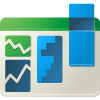
\includegraphics[scale=0.8]{images/einfuehrung/gft-logo} \\[0.3cm]

\includegraphics[scale=0.6]{images/einfuehrung/gft-text-logo}
\end{center}

\section{Was ist Google Fusion Tables?}
Google Fusion Tables ist eine Datenbank-Dienst in der \gls{Cloud}, welche von Google zur Verfügung gestellt wird.  Die Datenbank ist spezialisiert auf das Speichern und Visualisieren von geografischen Daten.
Der Dienst wurde am 10. Juni 2009 der Öffentlichkeit zugänglich gemacht\cite{fusion-table-announce}. Das erklärte Ziel dabei war es, die Nutzung einer Datenbank so einfach wie möglich zu machen.

\begin{figure}[!ht]
	\centering
	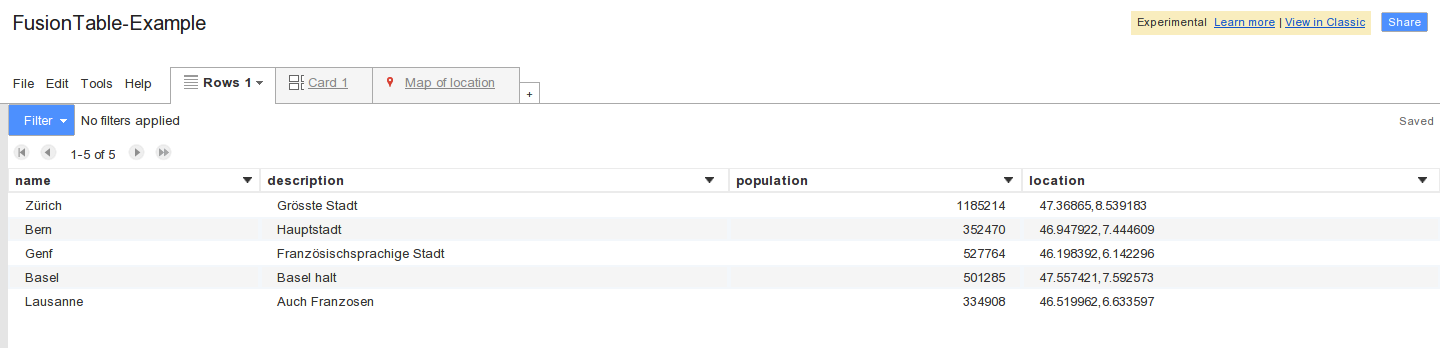
\includegraphics[width=\textwidth]{images/einfuehrung/gft-webgui-table}
	\caption{Tabellenansicht von Google Fusion Tables im Web-GUI}
	\label{gft-webgui-table}
\end{figure}

\begin{figure}[!ht]
	\centering
	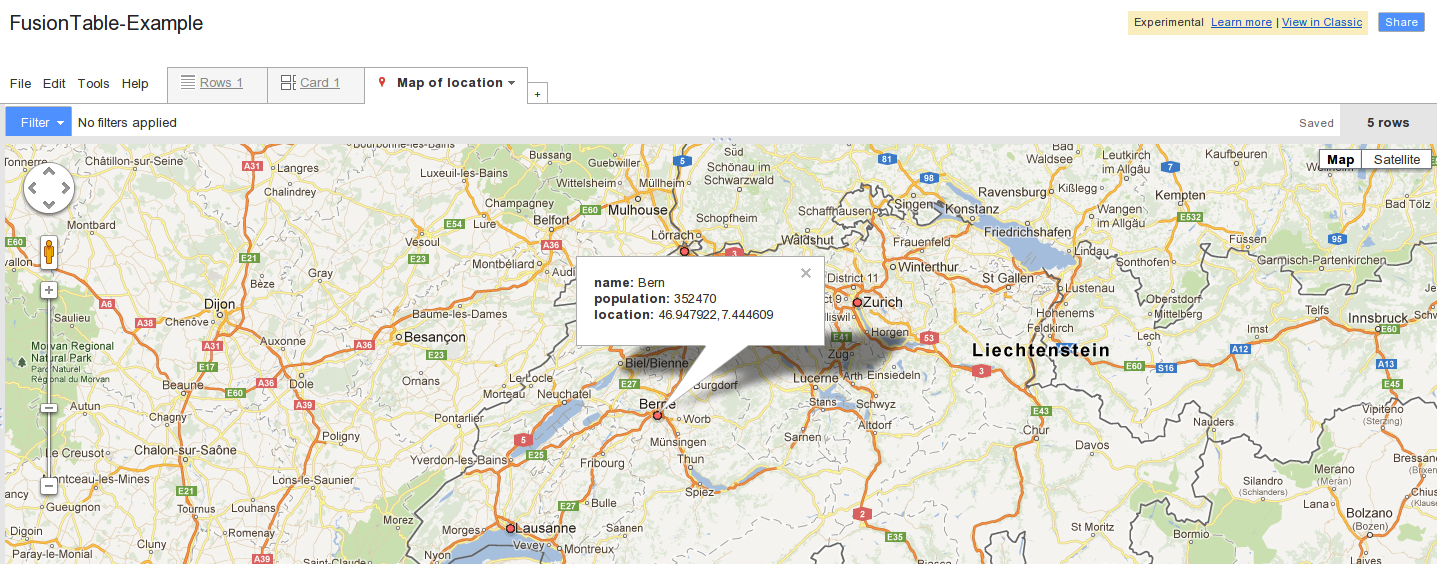
\includegraphics[width=\textwidth]{images/einfuehrung/gft-webgui-map}
	\caption{Kartenansicht von Google Fusion Tables im Web-GUI}
	\label{gft-webgui-map}
\end{figure}

\subsection{Kollaboration und Nutzung von öffentlichen Daten}
Der Gedanke der \gls{Cloud} lässt sich abseits vom Technischen noch weiterdenken. Durch die allgemeine Verfügbarkeit der Fusion Tables Datenbank, lassen sich die dort eingetragenen Daten mit anderen Benutzern oder gar der Öffentlichkeit teilen. Google bietet sogar die Möglichkeit öffentliche Tabellen zu durchsuchen\footnote{\url{https://www.google.com/fusiontables/search}}.

Tabellen können zudem mit anderen Tabellen gemerged werden, wodurch die Vereinigung der Daten wiederum neue Möglichkeiten zur Nutzung der Daten ermöglicht. Eine öffentlich zugängliche Tabelle mit Länderpolygonen lässt sich so beliebig oft gebrauchen, um Daten mit Ländern zu verknüpfen und diese dann auf einer Karte darzustellen.

Diese passive Kollaboration ermöglicht es, auf eine breite Palette an öffentlichen bzw. veröffentlichten Daten zurückzugreifen. Via Import lassen sich auch andere bereits bestehende Daten mit Fusion Tables nutzen. Unterstützt sind dabei Tabellen (via Google Spreadsheet), \gls{CSV} und \gls{KML} Dateien. Mit unserem im Kapitel \ref{converter-build} vorgestellten Build lassen sich eine breite Palette von Dateiformaten in Google Fusion Tables importieren.

Um aktiv zu kollaborieren, hat Google auch einige Features angedacht. So ist es möglich, einzelne Datensätze oder gar Zellen in der Tabelle zu kommentieren, sofern man die nötigen Berechtigungen dafür hat. Falls man Daten von mehreren Lieferanten verwalten lassen will, kann eine Partei eine Tabelle erstellen und verschiedene Views darauf erstellen, welche jeweils von den verschiedenen Datenlieferanten gepflegt werden. Durch entsprechend gesetzte Berechtigungen kann so jeder seine Daten zum Ganzen beitragen, ohne Zugriff auf die Daten von anderen Lieferanten zu haben. Einzig der Besitzer der Tabelle hat Berechtigungen auf alle Inhalte. Google hat als Beispiel für diesen Use Case die Applikation \emph{Flu Vaccine Finder} erstellt, welche es den Anbietern von Grippeimpfungen ermöglicht, ihre Lokale selbstständig zu erfassen und zu verwalten.\cite{data-gathering}

\subsection{Verschiedene Tabellenarten}
Google Fusion Tables unterscheidet grundsätzlich drei verschiedene Tabellenarten\footnote{Tabellenarten in Google Fusion Tables: \url{https://developers.google.com/fusiontables/docs/developers_guide\#Exploring}}. Jede Tabelle hat sowohl einen Namen wie auch eine numerische und \emph{verschlüsselte} ID (\inlinecode{encid}). Angesprochen wird die Tabelle ausschliesslich über deren ID, wobei das neue \gls{API} (siehe Abschnitt \ref{trusted-tester-api}) nur noch die \inlinecode{encid} akzeptiert.

\subsubsection{Base Table}
Eine normale Tabelle kann kann sowohl über das Web-GUI wie auch über das \gls{API} erstellt werden. Eine Tabelle kann Daten entweder von einer \gls{KML}- oder einer \gls{CSV}-Datei importieren oder von einer bereits vorhandenen Google Spreadsheet-Datei übernehmen.

\subsubsection{Merged Table}
\label{merge-table}
Merged Tables sind ein Mittel, um zwei Fusion Tables zusammenzuführen. Der Benutzer muss dabei Berechtigungen für beide Tabellen haben. Im \gls{Merge}-Dialog kann dann die \inlinecode{JOIN}-Spalte ausgewählt werden. Sobald der \gls{Merge}-Vorgang abgeschlossen ist, gibt es eine neue \emph{virtuelle} Tabelle, welche die Daten aus beiden zugrundeliegenden Tabellen enthält. Der \gls{Merge} führt dabei intern einen \inlinecode{LEFT OUTER JOIN} durch, wodurch alle Daten der Orginaltabelle erhalten bleiben, jedoch nur die Daten der zweiten Tabelle, welche dem \inlinecode{JOIN}-Kriterium entsprechen\footnote{ \url{https://developers.google.com/fusiontables/docs/developers_guide\#Terminology}}. Änderungen an den zugrundeliegenden Tabellen sind sofort sichtbar.

\begin{figure}[!ht]
	\centering
	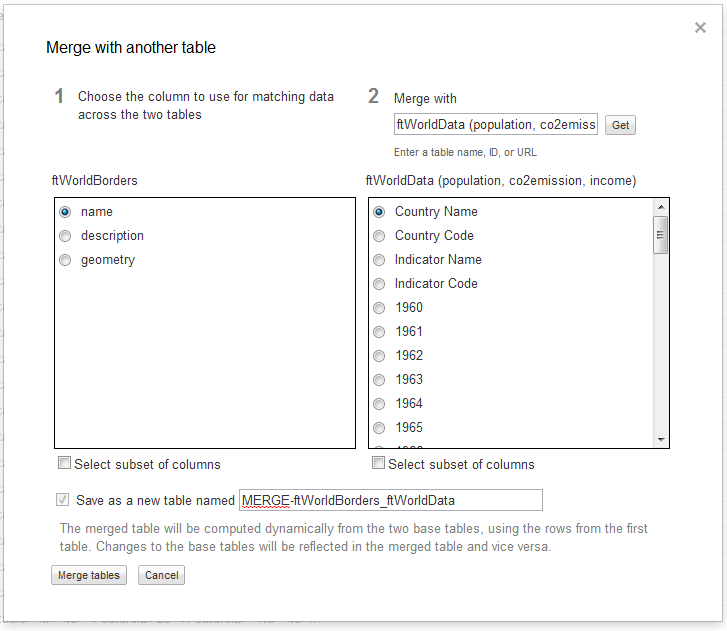
\includegraphics[width=0.7\textwidth]{images/usecase1-worlddata/documentation/worlddata-merge2}
	\caption{Erstellen einer Merged Table über das Web-GUI}
	\label{create-merge-table}
\end{figure}

Merged Tables haben einige Einschränkungen. So lassen sie sich bislang nicht via \gls{API} erstellen, sondern aussschliesslich über das Web-GUI. \inlinecode{INSERT}-Befehle sind nicht möglich und \inlinecode{UPDATE} nur auf Attributen, die nicht am Join beteiligt sind.

Wir haben die Merged Tables in unserer erstellen Webapplikation \emph{WorldData} verwendet (siehe Kapitel \ref{worlddata}).

\subsubsection{View}
Mit Views können Einschränkungen von Base Tables vorgenommen werden. Dies kann einserseits die Projektion betreffen, so dass eine View nicht mehr alle Attribute der Orginaltabelle beinhaltet. Andererseits aber auch die Daten selbst, nämlich dann, wenn eine Einschränkung (\inlinecode{WHERE}-Klausel) definiert wurde. Letzteres ist jedoch über das Web-GUI nicht möglich.

Views sind auch ein ideales Mittel, um die Berechtigungen zu steuern. So kann z.B. der lesende Zugriff auf eine Menge von Daten gewährt werden, jedoch der schreibende Zugriff nur auf eine Untermenge, indem man eine entsprechende View erstellt. Wir haben dieses Prinzip in unserem \emph{FixMyStreet} Use Case verwendet (siehe Kapitel \ref{fixmystreet})

Views können nur von Base Tables oder anderen Views erstellt werden, Merged Tables werden nicht unterstützt\footnote{\url{https://developers.google.com/fusiontables/docs/developers_guide\#CreatingView}}.

Ein schönes Beispiel für die Verwendung von Views in Google Fusion Tables ist der \emph{Flu Vaccine Finder}\footnote{\url{https://developers.google.com/fusiontables/docs/articles/data_gathering}} von Google selbst.

\subsection{Limiten}
Da die Google Fusion Tables kostenlos angeboten werden, hat Google einige Limiten bei der Benutzung der Datenbank festgelegt. So darf eine einzelne Tabelle maximal 250MB Speicher belegen. Zudem sind die Abfragen pro Benutzer und Tag auf 25'000 beschränkt. Auf der Karte lassen sich maximal 100'000 Elemente gleichzeitig darstellen. Allgemein werden zudem bei Abfragen nur die ersten 100'000 Datensätze der Datenbank für das Erstellen der Antwort berücksichtigt. Diese Einschränkungen können Kunden des Google Maps \gls{API} Premier\footnote{\url{http://www.google.com/enterprise/earthmaps/maps.html}} auf Anfrage verändern. Die Preise dafür starten bei \$10'000 pro Jahr und steigen je nach Bedürfnissen nach oben.\cite{fusion-tables-geo-limits}

\begin{longtable}{|l|l|}
\hline 
\textbf{Beschreibung} & \textbf{Limitation} \\ 
\hline 
Speicher pro Tabelle & 250MB \\ 
\hline 
Abfragen pro Benutzer und Tag & 25'000 \\ 
\hline 
Gleichzeitig angezeigte Elemente auf Karte & 100'000 \\ 
\hline 
Für Abfragen berücksichtigte Datensätze & erste 100'000 \\ 
\hline 
\caption{Limitationen der Google Fusion Tables}
\label{gft-limitations}
\end{longtable} 

\subsection{Austausch mit den Google Entwicklern}
\label{austausch-mit-google}
Da es sich bei Google Fusion Tables um ein relativ neues Projekt handelt, war uns bewusst, dass wir früher oder später vor Problemen stehen würden. Von daher war für uns klar, dass wir die beiden offiziellen Supportkanäle (Mailingliste\footnote{Die Mailingliste ist für allgemeine oder konzeptionelle Fragen: \url{https://groups.google.com/forum/?fromgroups\#!forum/fusion-tables-users-group}} und StackOverflow\footnote{Google hat alle technischen Fragen zu GFT in die bekannte Entwickler-Community StackOverflow ausgelagert: \url{http://stackoverflow.com/questions/tagged/google-fusion-tables}}) aktiv nutzen werden. Zum einen ist es sehr interessant zu sehen, welche Ideen und Probleme andere Entwickler haben, zum anderen konnten wir so einen guten Kontakt zur Community pflegen.

Hauptsächlich wendeten wir uns via Mailingliste an die Google Entwickler, wo man in der Regel innerhalb eines Tages sehr gute Antworten auf Fragen bekommt. Auch ein von uns gemeldeter Bug\footnote{Bug-Report \emph{COUNT() returns as NaN in Trusted Tester \gls{API}}: \url{http://code.google.com/p/fusion-tables/issues/detail?id=1086}} wurde sehr schnell behoben. Der Bug ist uns beim Wechsel auf das neue Trusted Tester \gls{API} (siehe Abschnitt \ref{trusted-tester-api}) dank unserer Unit-Tests aufgefallen. Leider gab es aber nicht für alle unsere Anfragen einfache Lösungen (siehe Abschnitt \ref{geocodierung-bug}).

Im April fand ein Google+ Hangout (Videokonferenz) mit zwei Google Fusion Tables Entwicklern zum Trusted Tester \gls{API} statt, wo Feedback und Anregungen gesammelt wurden. Da nicht viele Leute anwesend waren, konnten wir ausführlich Feedback geben und unsere Use Cases besprechen.

% SQL API
\section{SQL API}
\label{sql-api}
Das SQL API bietet eine Schnittstelle mit welcher man mit SQL-ähnlichen Befehlen Daten aus Google Fusion Tables abfragen oder verändern kann. Sie verfügt bereits über eine grosse Palette an möglichen Befehlen\footnote{Befehlsreferenz: \url{https://developers.google.com/fusiontables/docs/developers_reference}}. Die SQL-Befehle werden als Parameter in folgender Form an das API übergeben:

\url{https://www.googleapis.com/fusiontables/<apiVersion>/query?sql=<statement>}

Lesende Zugriffe (\inlinecode{SELECT}, \inlinecode{SHOW TABLES}, \inlinecode{DESCRIBE}) werden dabei als \inlinecode{GET}-Request geschickt, schreibende Zugriffe (\inlinecode{CREATE}, \inlinecode{DROP}, \inlinecode{INSERT}, \inlinecode{UPDATE}, \inlinecode{DELETE}) mit der \inlinecode{POST}-Methode. Um Daten zu schreiben und für den Zugriff auf private Tabelle ist eine Authentifizierung (siehe Abschnitt \ref{oauth}) mit OAuth nötig.

\begin{longtable}{|p{0.2\twocelltabwidth}|p{0.8\twocelltabwidth}|}
\hline 
\textbf{Befehl} & \textbf{Beschreibung} \\ 
\hline 
\inlinecode{SHOW TABLES} & Abfrage aller Tabellen des angemeldeten Benutzers \\ 
\hline 
\inlinecode{DESCRIBE} & Bezeichnung und Datentypen aller Spalten in einer Tabelle \\ 
\hline 
\inlinecode{CREATE TABLE} & Erstellen einer neuen Tabelle \\ 
\hline 
\inlinecode{CREATE VIEW} & Erstellen einer View auf Grundlage einer bestehenden Tabelle \\ 
\hline 
\inlinecode{SELECT} & Selektieren von Daten einer Tabelle \\ 
\hline 
\inlinecode{INSERT} & Neue Zeile zu einer Tabelle hinzufügen \\ 
\hline 
\inlinecode{UPDATE} & Daten in einer Tabelle verändern \\ 
\hline 
\inlinecode{DELETE} & Daten aus einer Tabelle löschen \\ 
\hline 
\inlinecode{DROP TABLE} & Löschen einer Tabelle \\ 
\hline 
\caption{Liste der verfügbaren SQL Befehle des SQL APIs}
\end{longtable}

\subsection{Abfragen (Queries)}
Mit dem \inlinecode{SELECT}-Befehl des SQL API lassen sich Abfragen an Google Fusion Tables stellen. Die untenstehende Tabelle gibt eine Übersicht der Möglichkeiten.

\begin{longtable}{|p{0.25\twocelltabwidth}|p{0.75\twocelltabwidth}|}
\hline 
\textbf{Bereich} & \textbf{Beschreibung} \\ 
\hline
Aggregation &  Folgende Funktionen sind unterstützt:
\begin{itemize}[noitemsep]
\item \inlinecode{COUNT()}
\item \inlinecode{SUM({\textless}column{\_}name{\textgreater})}
\item \inlinecode{AVERAGE({\textless}column{\_}name{\textgreater})}
\item \inlinecode{MAXIMUM({\textless}column{\_}name{\textgreater})}
\item \inlinecode{MINIMUM({\textless}column{\_}name{\textgreater})}
\end{itemize} \\ 
\hline 
Einschränkung auf Datensatz &  \inlinecode{ROWID = {\textless}id{\textgreater}} \\
\hline 
Einschränkung auf Attributen &  Für Zahlen: \inlinecode{{\textless}column{\_}name{\textgreater} {\textless}operator{\textgreater} {\textless}number{\textgreater}}
wobei \inlinecode{{\textless}operator{\textgreater}} folgende Werte haben kann: 
\begin{itemize}[noitemsep]
\item \inlinecode{{\textgreater}, {\textless},{\textgreater}=, {\textless}=, =}
\end{itemize}

Für Strings: \inlinecode{{\textless}column{\_}name{\textgreater} {\textless}operator{\textgreater} {\textless}string{\textgreater} }
wobei \inlinecode{{\textless}operator{\textgreater}} folgende Werte haben kann: 
\begin{itemize}[noitemsep]
\item \inlinecode{\textgreater, {\textless}, \textgreater=, {\textless}=, =}
\item \inlinecode{LIKE}
\item \inlinecode{MATCHES}
\item \inlinecode{STARTS WITH}
\item \inlinecode{ENDS WITH}
\item \inlinecode{CONTAINS}
\item \inlinecode{CONTAINS IGNORING CASE}
\item \inlinecode{DOES NOT CONTAIN}
\item \inlinecode{NOT EQUAL TO}
\item \inlinecode{IN}
\end{itemize} 

Formeln oder Vergleiche mit anderen Attributen der Tabelle sind nicht unterstützt.\\
\hline
Einschränkung auf Anzahl Datensätze & \inlinecode{LIMIT {\textless}number{\textgreater}} 
wobei \inlinecode{{\textless}number{\textgreater}} angibt wieviele Datensätze des Resultats zurückgeliefert werden sollen.


Mit \inlinecode{OFFSET {\textless}number{\textgreater}} kann der Bereich, ab welchem das Limit zählt verändert werden.
\\
\hline 
\caption{Liste der verfügbaren Abfragemöglichkeiten des SQL APIs}
\end{longtable}

Um mehrere Bedingungen in einer \inlinecode{WHERE}-Klausel zu verwenden können diese mit \inlinecode{AND} verbunden werden. Verknüpfungen mit \inlinecode{OR} werden hingegen nicht unterstützt.

\subsection{Ortsbezogene Abfragen (Spatial-Queries)}
\label{sqlapi-spatialqueries}
Das SQL API bieten zudem eine Reihe von speziellen ortsabhängigen Abfrage-Möglichkeiten, welche in der folgenden Tabelle dokumentiert sind.

\begin{longtable}{|p{0.25\twocelltabwidth}|p{0.75\twocelltabwidth}|}
\hline 
\textbf{Spatial Keyword} & \textbf{Beschreibung} \\ 
\hline 
\inlinecode{ST{\_}INTERSECTS( {\textless}location{\_}column{\textgreater}, {\textless}geometry{\textgreater} )} & Liefert alle Zeilen zurück, welche sich innerhalb der definierten Geometrie \inlinecode{{\textless}geometry{\textgreater}} befinden.

\begin{itemize}[noitemsep]
\item Als \inlinecode{{\textless}location{\_}column{\textgreater}} muss eine Spalte der Tabelle, vom Typ \emph{Location}, angegeben werden.
\item Als \inlinecode{{\textless}geometry{\textgreater}} kann entweder ein \inlinecode{CIRCLE} oder ein \inlinecode{RECTANGLE} verwendet werden. Ein \inlinecode{POLYGON}-Typ fehlt derzeit noch. 
\end{itemize}

\inlinecode{ST{\_}INTERSECTS} kann als Bedingung in der \inlinecode{WHERE}-Klausel des Statements verwendet werden.

\textit{Hinweis: \inlinecode{ST{\_}INTERSECTS} und \inlinecode{ST{\_}DISTANCE} dürfen nicht zusammen im gleichen Statement verwendet werden.} \\ 
\hline 
\inlinecode{ST{\_}DISTANCE( {\textless}location{\_}column{\textgreater}, {\textless}coordinate{\textgreater} )} & Liefert die Datensätze sortiert nach der Distanz zur angegebenen Koordinate \inlinecode{{\textless}coordinate{\textgreater}} zurück.

\begin{itemize}[noitemsep]
\item Als \inlinecode{{\textless}location{\_}column{\textgreater}} muss eine Spalte der Tabelle, vom Typ \emph{Location}, angegeben werden.
\item Die \inlinecode{{\textless}coordinate{\textgreater}} stellt die Koordinate dar, zu welcher der Abstand gemessen werden soll. 
\end{itemize}

\inlinecode{ST{\_}DISTANCE} kann als Bedingung in der \inlinecode{ORDER BY}-Klausel des Statements verwendet werden.

\textit{Hinweis: \inlinecode{ST{\_}INTERSECTS} und \inlinecode{ST{\_}DISTANCE} dürfen nicht zusammen im gleichen Statement verwendet werden.} \\ 
\hline 
\inlinecode{CIRCLE( {\textless}coordinate{\textgreater}, {\textless}radius{\textgreater} )} & Wird verwendet, um einen Kreis von der angegebenen Koordinate \inlinecode{{\textless}coordinate{\textgreater}} mit den Radius \inlinecode{{\textless}radius{\textgreater}} zu erhalten. \\ 
\hline 
\inlinecode{RECTANGLE( {\textless}coordinate{\_}1{\textgreater}, {\textless}coordinate{\_}2{\textgreater} )} & Wird verwendet um ein Rechteck mit den Ecken \inlinecode{{\textless}coordinate{\_}1{\textgreater}} (links oben) und \inlinecode{{\textless}coordinate{\_}2{\textgreater}} (rechts unten) zu erhalten. \\ 
\hline 
\caption{Liste der verfügbaren Spatial Queries des SQL APIs}
\end{longtable} 

\section{Client Libraries}
Google bietet Client Libraries zum \gls{API} in den Sprachen PHP\footnote{\url{http://code.google.com/p/fusion-tables-client-php/}} und Python\footnote{\url{http://code.google.com/p/fusion-tables-client-python/}} an. Da wir eine Webapplikation möglichst ohne Serverteil erstellen wollten, waren wir auf eine Bibliothek in JavaScript angewiesen. Da es bislang noch keine solche gab, haben wir selbst begonnen die GftLib zu entwickeln (siehe Abschnitt \ref{gftlib-js}).

Durch die Same-Origin-Policy\footnote{Die Same-Origin-Policy (SOP) ist ein Sicherheitskonzept, das es JavaScript und ActionScript nur dann erlaubt, auf Objekte einer anderen Webseite zuzugreifen, wenn sie aus derselben Quelle (Origin) stammen.\cite{sop} }, wurden wir daran gehindert \gls{AJAX}-Requests direkt auf das Google \gls{API} abzusetzen. Wir mussten eine Alternative finden, ohne eine Serverkomponente einzuführen.

Schliesslich fanden wir in den Google Groups ein inoffizielles \gls{JSONP} \gls{API}\footnote{\url{https://groups.google.com/forum/?hl=en&fromgroups\#!topic/fusion-tables-users-group/jCiFfqCgCWM}}, welches es erlaubt \gls{AJAX}-Requests auch über die eigene Domäne hinweg zu senden. Diese Methode funktionierte jedoch nur für lesende Zugriffe. 

Für die schreibenden Zugriffe haben wir als Workaround einen \emph{Relay-Dienst} geschrieben, welcher auf unserem Webserver lief. Der Dienst hat lediglich die Requests entgegengenommen und diese dann an das Google API weitergeleitet.

Als wir den Zugriff auf das Trusted Tester API (siehe Abschnitt \ref{trusted-tester-api}) bekommen haben, konnten wir den Serverteil wieder entfernen. Google hat dort die Möglichkeit hinzugefügt hat, direkt mit ihrem JavaScript API Client\footnote{Google APIs Client Library for JavaScript: \url{http://code.google.com/p/google-api-javascript-client/}} Requests ans API zu schicken, somit entfällt die Same-Origin-Policy Problematik.

\section{Trusted Tester API}
\label{trusted-tester-api}
Es gibt derzeit zwei verschiedene Versionen des APIs: eine frei öffentlich zugängliche und das sogenannte \emph{Trusted Tester API}, welche derzeit im Beta-Stadium ist und nur ausgewählten Personen zur Verfügung steht. Als wir im Sprint 2 davon erfahren haben, haben wir uns für einen Zugang beworben, welchen wir dann auch erhalten haben.

Das Trusted Tester API bietet einige Neuerungen zur alten Schnittstelle. Es handelt sich bei diesem API um eine Vorabversion der neuen Schnittstelle, welche zukünftig ebenfalls der Öffentlichkeit zur Verfügung stehen soll. Neben dem API gibt es auch eine zugehörige Mailingsliste, auf der die Entwickler von Google Fragen beantworten und Tipps geben.

Zu den Neuerungen des neuen APIs gehört, dass es auch eine \gls{REST}-Schnittstelle erhalten hat. Damit ist es zum einen möglich Tabelleninformationen abzufragen als auch ganz klassisch CRUD-Operationen auf dem API auszuführen. Da wir uns bemüht haben unsere Beispiele möglichst ohne Server-Code zu schreiben, konnten wir besonders davon profitieren, mit dem neuen API \inlinecode{POST}-Requests abzuschicken und so endlich auch Schreiboperationen direkt via Browser zu unterstützen.

Alle Request an das \gls{REST}-API haben die folgende Form: \\
\url{https://www.googleapis.com/fusiontables/<apiVersion>/<resourcePath>?<parameters>}

Folgende Ressourcen sind derzeit unterstützt:
\begin{itemize}
	\item Table
	\item Column
	\item Template
	\item Style
\end{itemize}

Eine \emph{Row} oder \emph{Query} Ressource fehlt noch. Um Abfragen zu machen muss nach wie vor das SQL API (siehe Abschnitt \ref{sql-api}) verwendet werden.

\begin{longtable}{|p{0.5\twocelltabwidth}|p{0.5\twocelltabwidth}|}
\hline 
\textbf{Ziel} & \textbf{HTTP Mapping} \\ 
\hline 
Alle Ressourcen eines Typs auflisten & \inlinecode{GET} auf einem Ressource-Typ\\ 
\hline 
Eine spezifische Ressource holen	& \inlinecode{GET} auf einer Ressource\\
\hline 
Eine neue Ressource einfügen (kreiert eine neue Ressource) & \inlinecode{POST} auf einem Ressource-Typ (mit Daten um eine neue Ressource zu erstellen)\\
\hline 
Aktualisieren einer bestehenden Ressource & \inlinecode{PUT} auf einer Ressource (mit Daten um die Ressource zu aktualisieren)\\
\hline 
Löschen einer Ressource & \inlinecode{DELETE}  auf einer Ressource\\
\hline 
\caption{HTTP Mapping des REST-APIs}
\end{longtable}


% Geocodierung
\section{Geocodierung in Google Fusion Tables}
\label{gft-geocoding}
Ein grosser Vorteil der Google Fusion Tables ist die automatische 
\gls{Geocodierung} von Standortdaten. Sobald eine neue Zeile via Web-GUI zu einer Tabelle hinzugefügt wird, werden alle Zellen vom Typ \emph{Location} einem eindeutigen Standort auf der Karte zugewiesen. Ist dies nicht möglich, da beispielsweise eine Adresse in mehreren Orten vorkommen kann, wird die Zelle nicht geocodiert und der Text wird gelb hinterlegt. In solchen Fällen hat man die Möglichkeit den zugehörigen Ort manuell mit Hilfe einer Karte zu wählen.

\begin{figure}[!ht]
	\centering
	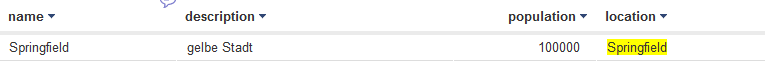
\includegraphics[width=\textwidth]{images/einfuehrung/geocoding_failed}
	\caption{Geocodierung für Ort Springfield fehlgeschlagen}
	\label{geocoding_failed}
\end{figure}

Die geocodierten Standorte werden als Metadaten in der Tabelle hinterlegt. Leider sind diese Daten über das SQL \gls{API} nicht selektierbar. Möchte man die erhaltenen Daten auf der Karte positionieren, so muss man für jede Zeile die \gls{Geocodierung} manuell vornehmen, was sich negativ auf die Ladezeit der Karte auswirkt.

\subsection{Geocoding-Dienste}
Es gibt verschiedene Dienste, welche eine solche \gls{Geocodierung} von Standortdaten anbieten. Die meisten davon haben aber eine Begrenzung der möglichen Anfragen pro Tag.

\begin{table}[H]
\centering
\begin{tabular}{|p{0.4\threecelltabwidth}|p{0.14\threecelltabwidth}|p{0.46\threecelltabwidth}|}
\hline 
\textbf{Anbieter} & \textbf{Anfragen pro Tag} & \textbf{URL} \\ 
\hline 
Google Maps Geocoding \gls{API} & 2500 & \url{https://developers.google.com/maps/documentation/geocoding/?hl=de} \\ 
\hline 
Yahoo! PlaceFinder \gls{API} & 50000 & \url{http://developer.yahoo.com/geo/placefinder/} \\ 
\hline 
MapQuest Geocoding \gls{API} & keine Begrenzung & \url{http://developer.mapquest.com/web/products/dev-services/geocoding-ws} \\ 
\hline 
\end{tabular}
\caption{Geocoding Limitierungen}
\end{table} 

\subsection{Geocoding von neuen Datensätzen}
\label{geocodierung-bug}
Ein grosses Problem stellt sich darin, dass neue Datensätze, welche über das SQL \gls{API} eingefügt wurden, nicht automatisch geocodiert werden. Dies führt dazu, dass diese Daten von Abfragen, welche eine ortsbezogene Einschränkung beinhalten (siehe Abschnitt \ref{sqlapi-spatialqueries}), nicht zurückgeliefert werden.

Eine \gls{Geocodierung} dieser Daten kann nur manuell über das Fusion Tables Web-GUI gestartet werden.

% Google Maps API - FusionTablesLayer
\section{Google Maps API - FusionTablesLayer}
\label{gmap-api-fusiontableslayer}
Google bietet von Haus aus bereits eine Fusion Table-Integration im Google Maps \gls{API} V3 an. Damit ist es möglich Fusion Tables als eigenständige Layer direkt auf der Karte darzustellen.
Die Möglichkeiten dieser Layer sind noch stark eingeschränkt, die grundlegenden Funktionalitäten für das Arbeiten mit Geodaten sind aber bereits vorhanden.

So ist es möglich, Abfragen mit \inlinecode{WHERE}-Conditions einzuschränken oder die Stile des Layers selbst zu bestimmen.

\subsection{Karten-Stile}
\label{fusiontableslayer-styles}
Die FusionTablesLayer bieten ein abfragebasiertes Styling der Ebene an. Damit ist es möglich, Flächen oder Linien farblich hervorzuheben oder andere Icons für Markierung zu verwenden. Zu jedem Stil kann man eine Einschränkung festlegen, welche bestimmt, ob dieser für den aktuellen Datensatz angewendet wird oder nicht. Die Einschränkung entspricht grundsätzlich einer \inlinecode{WHERE}-Condition in der Abfrage.

\emph{Hinweis: Passen mehrere Einschränkungen auf einen Datensatz, erhält dieser den Stil, welcher als letztes definiert wurde. Dies kann zu ungewollten Resultaten führen.}

\subsubsection{Beispiel eines Stils:}
\lstset{language=JavaScript}
\begin{lstlisting}[caption=Beispiel eines FusionTablesLayer-Stylings, label=fusiontableslayers-styles-example]
styles: [{
	polygonOptions: {
		fillColor: "#00FF00", // gruen
		fillOpacity: 0.3
	}
}, {
	where: "birds > 300",
	polygonOptions: {
		fillColor: "#0000FF" // blau
	}
}]
\end{lstlisting}

In diesem Beispiel\footnote{Quelle: \url{https://developers.google.com/maps/documentation/javascript/layers?hl=de-DE\#fusion_table_styles} (Stand: 21.05.2012)} werden alle Polygone der Tabelle, welche in der Spalte \emph{birds} eine Zahl grösser als 300 eingetragen haben, \emph{blau} eingefärbt. Die restlichen Polygone erhalten eine \emph{grüne} Färbung mit einer Deckkraft von 30\%.

\subsubsection{Einschränkungen}
\label{fusiontableslayer-styles-restrictions}
Das Google Maps \gls{API} hat momentan folgende Einschränkungen bezüglich den Ebenenstilen definiert.

\begin{table}[H]
\centering
\begin{tabular}{|l|l|}
\hline 
\textbf{Beschreibung} & \textbf{Limitation} \\ 
\hline 
Anzahl Ebenen pro Karte & 5 \\ 
\hline 
Anzahl Ebenen, auf denen Stile definiert sein dürfen & 1 \\ 
\hline 
Anzahl Stile auf Ebene & 5 \\ 
\hline 
\end{tabular} 
\caption{Limitationen der Stile auf Fusion Table-Ebenen}
\label{fusiontableslayer-stlyes-limitations}
\end{table}

\subsection{Heatmaps}
Ein weiteres Feature der Fusion Table-Ebenen ist die Möglichkeit, die Daten der Tabelle direkt als Heatmap darzustellen. Dabei werden die Daten automatisch nach der Häufigkeit der Vorkommnisse an einem Ort anders eingefärbt. Der verwendete Farbverlauf geht dabei von \emph{grün} (für wenig Daten) bis \emph{rot} (für viele Daten).

\begin{figure}[!ht]
	\centering
	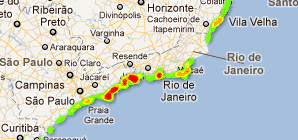
\includegraphics{images/einfuehrung/gmap_fusiontableslayer_heatmap}
	\caption{Daten als Heatmap mit FusionTablesLayer}
	\label{fusiontableslayer-heatmap}
\end{figure}

Leider sind momentan die Konfigurationsmöglichkeiten der Heatmap auf ein Minimum beschränkt. Eine Legende lässt sich beispielsweise nicht anzeigen. So kann man nicht genau sagen, welche Werte nun hinter den verschiedenen Farben stecken. Zudem lassen sich diese auch nicht verändern.

\subsection{Performance}
Der grösste Vorteil der Fusion Table-Ebenen steckt aber nicht zwingend in den sichtbaren Features. Man findet ihn wohl eher darin, dass die Geocodierungen der Standort-Daten direkt aus der Tabelle gelesen werden und nicht manuell vom Client abgefragt werden müssen. Dadurch kann die Ebene komplett auf den Servern von Google aufbereitet werden. Der Client muss die erhaltenen Daten lediglich noch darstellen. Der Vorteil davon wird durch das Diagramm \ref{fusiontableslayer-compare_markers}\footnote{Quelle: \url{http://www.google.com/events/io/2011/sessions/managing-and-visualizing-your-geospatial-data-with-fusion-tables.html} (Stand: 17.05.2012)} schnell ersichtlich.

\begin{figure}[!ht]
	\centering
	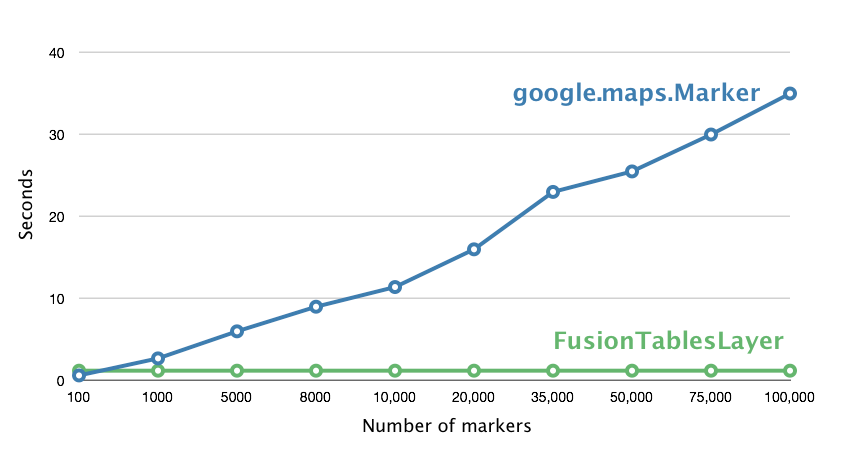
\includegraphics[width=0.9\textwidth]{images/einfuehrung/gmap_fusiontableslayer_vs_markers}
	\caption{FusionTablesLayer verglichen mit Markers}
	\label{fusiontableslayer-compare_markers}
\end{figure}

Die Zeit für das Rendering der Karte bleibt demnach bei der Verwendung von Fusion Table-Ebenen konstant und somit unabhängig von der Anzahl Markierungen, welche gesetzt werden müssen. Der Rechenaufwand, der für das Erstellen der JavaScript Marker-Objekte verwendet werden müsste, wird direkt von den Google Servern übernommen und das Resultat als Bild zum Client gesendet. Daraus resultiert die konstante Zeit, welche für die Anfrage zum Server und für das Senden der Antwort zum Client verwendet wird.

\subsection{Einschränkungen}
\subsubsection{Freigabe der Tabelle}
Ein grosser Nachteil der Fusion Table-Ebenen besteht darin, dass die verwendeten Fusion Tables als  \emph{öffentlich} markiert sein müssen, um diese auf einer Karte darzustellen. Dies bedeuted, dass jeder die Tabellen anzeigen oder auslesen kann. Es ist also nicht möglich, eine Tabelle mit sensiblen Daten als Fusion Table-Ebene darzustellen.

Von Google wird zur Lösung dieses Problems aber folgendes Vorgehen vorgeschlagen: Man kann für Tabellen mit sensiblen Inhalten eine View erstellen, welche lediglich die öffentlichen Spalten und Zeilen selektiert. Diese View könnte man dann als \emph{öffentlich} markieren und in einer Fusion Table-Ebene verwenden.

Eine Ausnahme dieser Regelung bilden dabei die Maps \gls{API} Premier Kunden. Diese haben die Möglichkeit eine Fusion Table als \emph{Protectet Map Layer} freizugeben, wodurch sich diese nur in einer definierten Applikation als Ebene einbinden lässt. Die Tabelle bleibt dabei komplett privat und kann nicht ausgelesen werden.

\subsubsection{Event-Handling auf Fusion Table-Ebenen}
Bislang ist es erst möglich, den Klick-Event auf einer Fusion Table-Ebene zu behandeln. Dieser liefert standardmässig das HTML-Template des InfoWindows mit. Zudem erhält man die Daten der "`angeklickten Zeile"' beziehungsweise die zugehörigen Daten des angeklickten Objekts auf der Karte. Man hat die Möglichkeit, dieses Template anzupassen bevor das InfoWindow angezeigt wird.

Weitere Events können auf einer Fusion Table-Ebene aber noch nicht behandelt werden. Es ist also nicht möglich, beispielsweise ein Objekt auf der Karte bei einem MouseOver-Event anders einzufärben oder ähnliches.

Diese fehlenden Möglichkeiten wurden schon oft von anderen FusionTables-Benutzern bei den Google-Entwicklern angefordert, welche dies ebenfalls als ein wichtiges Feature sehen, das noch implementiert werden muss.

Als Übergangslösung findet sich bereits eine Custom Library mit dem Namen \emph{Fusion Tips}\footnote{\url{http://gmaps-utility-gis.googlecode.com/svn/trunk/fusiontips/docs/examples.html}}. Diese legt über die Fusion Table-Ebene eine weitere transparente Ebene. Auf dieser Ebene kann man alle Events, welche das Google Maps \gls{API} anbietet, behandeln. Sobald die Maus über die Position eines Elementes auf der Fusion Table fährt, sendet der Event einen Request über das SQL \gls{API} an die Fusion Table und holt sich die Informationen zu der entsprechenden Zeile. So ist es möglich, ein neues Element mit der gleichen Form, aber beispielsweise einer anderen Farbe darüber zu legen.

Für den Benutzer entsteht so der Effekt, als würde sich die Farbe des gehoverten Elementes ändern.

Die Libary wird in folgendem Blog-Artikel sehr gut erklärt: \url{http://csessig.wordpress.com/2012/02/07/multiple-layers-and-rollover-effects-for-fusion-table-maps/}

\subsubsection{Weitere Einschränkungen}
Zusätzlich sind die allgemeinen Limitationen der Google Fusion Tables (siehe Tabelle \ref{gft-limitations}) zu beachten.


% Google Fusion Table Javascript Library (GftLib)
\section{Google Fusion Table Javascript Library (GftLib)}
\label{gftlib-js}
Die Google Fusion Table Library (GftLib) ist eine von uns entwickelte JavaScript-Bibliothek, welche die Kommunikation mit dem Google Fusion Table SQL API (siehe Abschnitt \ref{sql-api}) vereinfacht. Sie hilft dabei SQL-Abfragen zu erstellen und per \gls{AJAX} an das API zu versenden. Zudem kümmert sich die Library um die Authentifizierung via \gls{OAuth}, so dass auch schreibende Zugriffe oder Zugriffe auf private Tabellen möglich sind.

Die Bibliothek hat Abhängigkeiten zu jQuery\footnote{\url{http://jquery.com/}} (für einige Hilfsfunktionen) sowie dem Google API JavaScript Client\footnote{\url{http://code.google.com/p/google-api-javascript-client/}} (für die Authentifizierung und das Abschicken der Requests).

Die Bibliothek besteht aus 2 Klassen (GftLib und SqlBuilder). Die GftLib ist das API zum Client und steuert dementsprechend die Requests und die Authentifizierung. Der SqlBuilder ist eine Hilfsklasse, welche es erlaubt auf einfach Art und Weise SQL Befehle zu generieren.

\subsection{Beispiel}
In folgendem Beispiel sieht man die GftLib und den SqlBuilder im Einsatz. Zuerst werden alle benötigten Werte initialisiert (Zeilen 1-4), dann wird die Ausgabefunktion \inlinecode{printer} definiert, welche später als Callback-Funktion dient für den Request. Das heisst, dass die Funktion aufgerufen wird, sobald die Antwort der Abfrage zurückkommt. 

Mit der Funktion \inlinecode{convertToObject()} wird die Antwort von Google Fusion Tables in eine für den Benutzer angenehmere Form umgewandelt. Das Resultat der Fusion Tables kommt in der Form eines zweidimensionalen Arrays zurück, jeweils für jeden Datensatz alle abgefragten Felder. Die Funktion erstellt jeweils pro Datensatz ein Objekt, welches die angefragten Felder als Properties hat. So kann man mit deren Namen auf ihre Werte zugreifen (z.B. \inlinecode{places[i].name} oder \inlinecode{places[i].population}).

In diesem Beispiel wird das SQL Query direkt in der Funktion \inlinecode{execSelect()} erzeugt, welche dazu den SqlBuilder verwendet.

\lstset{language=JavaScript}
\begin{lstlisting}
var tableId = '1LWXSMsZINyfjAKGqeS-822wi4WmlaGmmvh20Ujw';
var gft = new GftLib();
var resultList = document.getElementById("result");

var printer = function(data) {
	var places = gft.convertToObject(data);

	for (var i = 0; i < places.length; i++) {
		var listElem = document.createElement('li');
		listElem.innerHTML = 'Place: ' + places[i].name + ' / Population: ' + places[i].population;
		resultList.appendChild(listElem);
	}
}

gft.execSelect(printer, {table:tableId, fields:['name', 'population']});
\end{lstlisting}

\subsection{Abhängigkeiten}
\begin{longtable}{|l|p{2cm}|p{7cm}|}
\hline 
\textbf{Library} & \textbf{Version} & \textbf{Verwendung} \\ 
\hline 
jQuery & 1.7.1-min & Helper-Funktionen und \gls{AJAX}-Requests für den OAuthTokenService  \\ 
\hline 
Google APIs Client Library & ALPHA release & \gls{AJAX}-Requests an das Google API und Authentifizierung \\ 
\hline 
\end{longtable} 

\subsection{Methoden}
\subsubsection{GftLib}
\begin{longtable}{|p{4.2cm}|p{3cm}|p{7cm}|}
\hline 
\textbf{Methode} & \textbf{Beschreibung} & \textbf{Parameter} \\ 
\hline 
\inlinecode{execQuery( callback, query )} &  Führt eine SQL-Abfrage aus & 
\begin{itemize}[noitemsep, nosep, leftmargin=12pt, before*={\mbox{}\vspace{-\baselineskip}}, after*={\mbox{}\vspace{-\baselineskip}}]
\item \inlinecode{callback} (Funktion): Callback-Methode welche nach Beendigung der Methode aufgerufen wird. 
\item \inlinecode{query} (String): SQL-Query
\end{itemize} \\ 
\hline 
\inlinecode{execSql( callback, sql )} & Führt einen beliebigen SQL-Befehl aus & 
\begin{itemize}[noitemsep, nosep, leftmargin=12pt, before*={\mbox{}\vspace{-\baselineskip}}, after*={\mbox{}\vspace{-\baselineskip}}]
\item \inlinecode{callback}: Callback-Methode welche nach Beendigung der Methode aufgerufen wird. 
\item \inlinecode{sql}: SQL-Befehl
\end{itemize} \\ 
\hline 
\inlinecode{execSelect( callback, options )} & Führt eine \inlinecode{SELECT}-Abfrage aus & 
\begin{itemize}[noitemsep, nosep, leftmargin=12pt, before*={\mbox{}\vspace{-\baselineskip}}, after*={\mbox{}\vspace{-\baselineskip}}]
\item \inlinecode{callback}: Callback-Methode welche nach Beendigung der Methode aufgerufen wird.
\item \inlinecode{options}: Parameter-Objekt für \inlinecode{SqlBuilder.selectStmt()}
\end{itemize} \\ 
\hline
\inlinecode{execInsert( callback, options )} & Führt einen \inlinecode{INSERT}-Befehl aus & 
\begin{itemize}[noitemsep, nosep, leftmargin=12pt, before*={\mbox{}\vspace{-\baselineskip}}, after*={\mbox{}\vspace{-\baselineskip}}]
\item \inlinecode{callback}: Callback-Methode welche nach Beendigung der Methode aufgerufen wird.
\item \inlinecode{options}: Parameter-Objekt für \inlinecode{SqlBuilder.insertStmt()}
\end{itemize} \\ 
\hline
\inlinecode{execUpdate( callback, options )} & Führt einen \inlinecode{UPDATE}-Befehl aus &
\begin{itemize}[noitemsep, nosep, leftmargin=12pt, before*={\mbox{}\vspace{-\baselineskip}}, after*={\mbox{}\vspace{-\baselineskip}}]
\item \inlinecode{callback}: Callback-Methode welche nach Beendigung der Methode aufgerufen wird. 
\item \inlinecode{options}: Parameter-Objekt für \inlinecode{SqlBuilder.updateStmt()}
\end{itemize} \\ 
\hline 
\inlinecode{execDelete( callback, options )} & Führt einen \inlinecode{DELETE}-Befehl aus & 
\begin{itemize}[noitemsep, nosep, leftmargin=12pt, before*={\mbox{}\vspace{-\baselineskip}}, after*={\mbox{}\vspace{-\baselineskip}}]
\item \inlinecode{callback}: Callback-Methode welche nach Beendigung der Methode aufgerufen wird.
\item \inlinecode{options}: Parameter-Objekt für \inlinecode{SqlBuilder.deleteStmt()} 
\end{itemize} \\ 
\hline 
\inlinecode{getTableDescription( callback, options )} & Führt eine \inlinecode{DESCRIBE}-Abfrage aus & 
\begin{itemize}[noitemsep, nosep, leftmargin=12pt, before*={\mbox{}\vspace{-\baselineskip}}, after*={\mbox{}\vspace{-\baselineskip}}]
\item \inlinecode{callback}: Callback-Methode welche nach Beendigung der Methode aufgerufen wird. 
\item \inlinecode{options}: Parameter-Objekt für \inlinecode{SqlBuilder.describeStmt()}
\end{itemize} \\
\hline 
\inlinecode{createView( callback, options )} & Führt einen \inlinecode{CREATE VIEW}-Befehl aus & 
\begin{itemize}[noitemsep, nosep, leftmargin=12pt, before*={\mbox{}\vspace{-\baselineskip}}, after*={\mbox{}\vspace{-\baselineskip}}]
\item \inlinecode{callback}: Callback-Methode welche nach Beendigung der Methode aufgerufen wird. 
\item \inlinecode{options}: Parameter-Objekt für \inlinecode{SqlBuilder.createViewStmt()} 
\end{itemize} \\ 
\hline 
\inlinecode{convertToObject( gftData )} & Konvertiert das Resultat einer Abfrage in sprechende Objekte & 
\begin{itemize}[noitemsep, nosep, leftmargin=12pt, before*={\mbox{}\vspace{-\baselineskip}}, after*={\mbox{}\vspace{-\baselineskip}}]
\item \inlinecode{gftData}: Antwort auf einen SQL Befehl von Google Fusion Tables
\end{itemize} \\ 
\hline 
\end{longtable} 

\subsubsection{SqlBuilder}
Die Methoden des SqlBuilders nehmen jeweils ein Parameter-Objekt\footnote{\url{http://www.refactoring.com/catalog/introduceParameterObject.html}} entgegen und erstellen daraus SQL-Befehle, welche dann als Input für die GftLib gebraucht werden können.

\begin{longtable}{|p{4.2cm}|p{3cm}|p{7cm}|}
\hline 
\textbf{Methode} & \textbf{Beschreibung} & \textbf{Parameter} \\ 
\hline
\inlinecode{selectStmt( options )} & Generiert ein \inlinecode{SELECT} Statement & 
\inlinecode{options}: Parameter-Objekt mit folgenden Feldern:
\begin{itemize}[noitemsep]
\item \inlinecode{fields}: Array von Feldernamen (Default *)
\item \inlinecode{table}: ID der Tabelle oder View
\item \inlinecode{conditions}: Array von Bedingungen für die \inlinecode{WHERE}-Klausel 
\end{itemize}\\
\hline
\inlinecode{insertStmt( options )} & Generiert ein \inlinecode{INSERT} Statement & 
\inlinecode{options}: Parameter-Objekt mit folgenden Feldern:
\begin{itemize}[noitemsep]
\item \inlinecode{fields}: Array von Feldernamen (Default *)
\item \inlinecode{table}: ID der Tabelle oder View
\item \inlinecode{values}: Array von Werten (in der gleichen Reihenfolge wie \inlinecode{fields})
\end{itemize}\\
\hline
\inlinecode{updateStmt( options )} & Generiert ein \inlinecode{UPDATE} Statement & 
\inlinecode{options}: Parameter-Objekt mit folgenden Feldern:
\begin{itemize}[noitemsep]
\item \inlinecode{fields}: Array von Feldernamen (Default *)
\item \inlinecode{table}: ID der Tabelle oder View
\item \inlinecode{values}: Array von Werten (in der gleichen Reihenfolge wie \inlinecode{fields})
\item \inlinecode{conditions}: Array von Bedingungen für die \inlinecode{WHERE}-Klausel
\end{itemize}\\
\hline
\inlinecode{deleteStmt( options )} & Generiert ein \inlinecode{DELETE} Statement & 
\inlinecode{options}: Parameter-Objekt mit folgenden Feldern:
\begin{itemize}[noitemsep]
\item \inlinecode{table}: ID der Tabelle oder View
\item \inlinecode{conditions}: Array von Bedingungen für die \inlinecode{WHERE}-Klausel
\end{itemize}\\
\hline
\inlinecode{describeStmt( options )} & Generiert ein \inlinecode{DESCRIBE} Statement & 
\inlinecode{options}: Parameter-Objekt mit folgenden Feldern:
\begin{itemize}[noitemsep]
\item \inlinecode{table}: ID der Tabelle oder View
\end{itemize}\\
\hline
\inlinecode{createViewStmt( options )} & Generiert ein \inlinecode{CREATE VIEW} Statement & 
\inlinecode{options}: Parameter-Objekt mit folgenden Feldern:
\begin{itemize}[noitemsep]
\item \inlinecode{viewName}: Name der neuen View
\item \inlinecode{query}: Ein SQL-Query, das der View zugrunde liegt
\end{itemize}\\
\hline
\end{longtable}

\subsection{Implementation}
\begin{figure}[H]
	\centering
	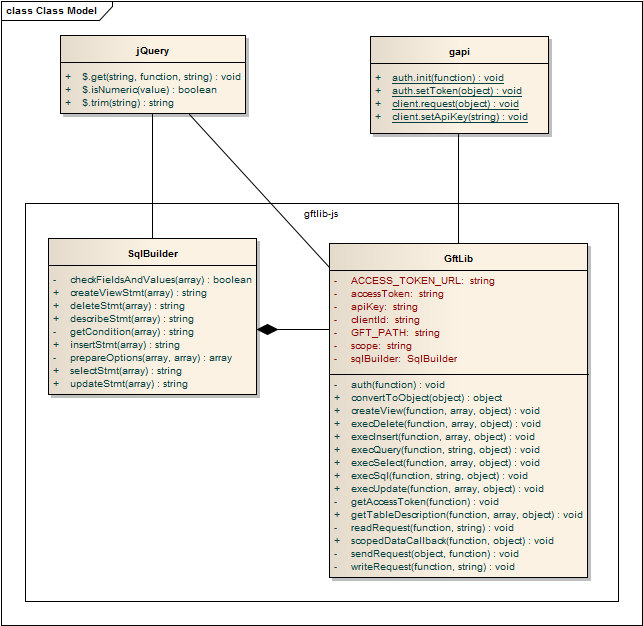
\includegraphics[width=\textwidth]{images/gftlib-js/gftlibjs-classmodel}
	\caption{GftLib Klassendiagramm}
	\label{gftlibjs-classmodel}
\end{figure}
\todo[inline]{GftLib: Implementierung?}

% Authentifizierung mit OAuth
\section{Authentifizierung mit OAuth}
\label{oauth}
\todo[inline]{OAuth Abschnitt schreiben}